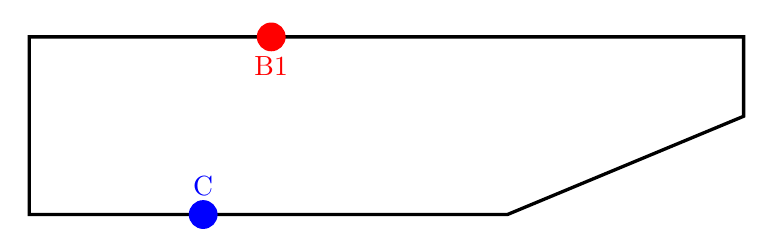
\begin{tikzpicture}[scale=0.06]
%\draw[help lines] (0,0) grid (142,-28);
\colorlet{Grey}{black!20}
%% External perimeter of the harbour
\draw[very thick] (0,0) -- (151.2,0)
	-- (151.2,-16.8) -- (151.2-50,-37.6)
	-- (0,-37.6) -- cycle;

%% Bateau
%\draw (46.4+4.8,0) circle[radius=5pt];
\node[mark size=5pt,color=red] at (46.4+4.8,0) {\pgfuseplotmark{*}};
\node[below,color=red] at (46.4+4.8,0-2) {B1};
%% Camion
\node[mark size=5pt,color=blue] at (4.8+32,-37.6) {\pgfuseplotmark{*}};
\node[above,color=blue] at (4.8+32,-37.6+2) {C};
\end{tikzpicture}